%% ------------------------------------------------------------------- %%
\chapter{Estado del Arte}
\label{cap:estadodelarte}
\lhead{\emph{Estado del Arte}} 

En este capítulo presentaremos los resultados de la Revisión Sistemática de la Literatura (RSL) referente a los métodos de detección de neo antígenos con técnicas de \textit{deep learning} y desde una perspectiva en las ciencias de la computación.

%% ------------------------------------------------------------------- %%
%% ------------------------------------------------------------------- %%
%% ------------------------------------------------------------------- %%
%% ------------------------------------------------------------------- %%

\section{Revisión Sistemática de la Literatura (RSL)}

Con el objetivo de mapear las principales técnicas de detección de  neo antígenos, se planteó desarrollar una Revisión Sistemática de la Literatura (RSL). La RSL, se enfocó en los métodos basados en \textit{deep learning} y desde una perspectiva de las ciencias de la computación. Se definió este objetivo, porque en la literatura ya existían varios otros \textit{reviews}, enfocados en el proceso general de vacunas personalizadas, y detección de neo antígenos. En esta sección, se describe el proceso que se llevó a cabo y sus resultados.


\subsection{Cadenas de busqueda y bases de datos}

En la Tabla \ref{tab:key_words}, se presentan las cadenas de búsqueda utilizadas para la RSL. Generalmente los términos sinónimos a \textit{neoantigen} utilizados en la literatura son \textit{peptide} y \textit{epitope}. Luego, algunos trabajos se enfocan en predecir el enlace entre un péptido y la molécula MHC, pero para células humanas la molécula MHC tiene el nombre de HLA. Además, hay varias clases como MHC-I y MHC-II. Debido a eso, se tenía que considerar todos esos sinónimos de MHC. También, otra diferencia existe en el término ``enlace'', del enlace péptido con MHC, algunos trabajos se refieren a él con los términos: \textit{binding}, \textit{presentation}, \textit{prediction} y \textit{detection}. Finalmente, algunos trabajos se enfocan en otra fase de la detección de neo antígenos, esta consiste en predecir el enlace entre el compuesto pMHC y T-cell Receptor (TCR) de las células T.

Luego, se utilizó Google Schoolar y Mendeley como motores de búsqueda al ser estos unos motores que indexan casi la totalidad de artículos científicos. Utilizando estas herramientas, se obtuvo artículos de las bases de datos descritas en la Tabla \ref{tab:bd_RSL}.




\begin{table}[H]
	\begin{center}
		\caption{Cadenas de busqueda utilizadas en la RSL.}
		\label{tab:key_words}
		\setlength{\tabcolsep}{0.5em} % for the horizontal padding
		{\renewcommand{\arraystretch}{1.4}% for the vertical padding
				\begin{tabular}{p{14cm}}
				\textbf{Cadena de busqueda} \\ \hline
				neoantigen  AND (detection OR pipeline) AND deep learning                                                                               \\
				(MHC OR HLA) AND binding  AND deep learning                                                                                             \\				
				(MHC-I OR MHC-II OR MHC OR HLA) AND (peptide OR epitope) AND ( binding OR affinity OR prediction OR detection OR presentation)          \\
				TCR interaction prediction                                                                                                              \\		
			\end{tabular}
		}
	\end{center}
\end{table}

\begin{table}[H]
	\begin{center}
		\caption{Bases de datos utilizadas en la RSL.}
		\label{tab:bd_RSL}
		\setlength{\tabcolsep}{0.5em} % for the horizontal padding
		{\renewcommand{\arraystretch}{1.2}% for the vertical padding
			\begin{tabular}{p{14cm}}
				\textbf{Bases de datos} \\ \hline
				IEEE Xplore                                                                               \\
				Science Direct \\				
				Springer          \\
				ACM Digital Library                                                                                                             \\	
				PubMed \\ 
				BioRxiv \\ 	
			\end{tabular}
		}
	\end{center}
\end{table}

\subsection{Selección de artículos}

Con las cadenas de búsqueda y considerando solo los artículos desde el 2018, se analizó el título de cada artículo encontrado por los motores de búsqueda y se seleccionaron 334 artículos. En la Tabla \ref{tab:number_papers}, se presenta la cantidad de artículos publicados por año. Para el caso del 2022, solo se tienen 57 artículos porque esta tesis se redactó a mediados del año 2022. 

Del total de artículos encontrados (342), se seleccionó un subconjunto basado en los criterios de inclusión y exclusión presentados de la Tabla  \ref{tab:criterios}. Estos criterios incluían que el artículo pertenezca a un \textit{conference} o \textit{journal} reconocido, que tenga una metodología detallada y que pertenezca al area de ciencia de la computación. Luego, en la Tabla \ref{tab:criterios}, se puede ver que hay un puntaje según cada criterio de inclusión, se utilizó este puntaje para calificar cada artículo y luego se seleccionaron los artículos que tenían un puntaje mayor a 4. En este proceso, se analizó el \textit{abstract} de los artículos y ciertas partes importantes según era necesario para asignar el puntaje. Al finalizar esta etapa, se obtuvieron 253 artículos, estos son los trabajos que se han analizado en la RSL. Adicionalmente, a los artículos seleccionados, se han considerado otros trabajos importantes que proponian bases de datos, \textit{pipelines} y \textit{reviews}.




\begin{table}[H]
	\begin{center}
		\caption{Cantidad de artículos encontrados y seleccionados según los criterios de inclusión y exclusión en la RSL.}
		\label{tab:number_papers}
		\setlength{\tabcolsep}{0.5em} % for the horizontal padding
		{\renewcommand{\arraystretch}{1.2}% for the vertical padding
			\begin{tabular}{ccc}
					\textbf{Año} & \textbf{Artículos encontrados} & \textbf{Artículos seleccionados}\\ \hline
				    2018 & 53 & 42 \\
				    2019 & 79 & 52 \\
				    2020 & 81 & 67 \\
				    2021 & 64 & 51 \\
				    2022 & 57 & 41 \\ \hline
				    Total & \textbf{342} & \textbf{253} \\
			\end{tabular}
		}
	\end{center}
\end{table}

\begin{table}[H]
	\begin{center}
		\caption{Criterios de inclusión y exclusión de artículos utilizados en la RSL.}
		\label{tab:criterios}
		\setlength{\tabcolsep}{0.5em} % for the horizontal padding
		{\renewcommand{\arraystretch}{1.2}% for the vertical padding
			\begin{tabular}{p{5.5cm}p{5.5cm}c}
				\textbf{Criterios de inclusión}                                                   & \textbf{Criterios de exclusión}                                                          & \textbf{Puntaje} \\ \hline
				Artículos con categoría ERA (A, B o C) si son conferencias y Journals Q1, Q2 o Q3. & No considerar los trabajos de baja calidad, que no esten rankeados.                       & 3                \\
				Trabajos que se basen en \textit{deep learning} para la detección de neo antígenos.          & Trabajos que se basan en el uso de alguna herramienta (investigaciónes realizadas por cientificos de otras areas). & 2                \\
				La metodología es detallada.                                                       &                                                                                          & 2                \\
				Tiene resultados clínicos                                                         &                                                                                          & 2                \\
				Tiene repositorio de código fuente.                                          &                                                                                          & 1                \\
				Comparte la base de datos utilizada.                                         &                                                                                          & 1               
			\end{tabular}
		}
	\end{center}
\end{table}





\section{Resultados de la RSL}\index{} 
\label{sec:neoantigen}


 El proceso para la detección de neo antígenos, es complejo, y generalmente consiste en: (1) extracción del tejido tumoral y secuenciamiento, (2) identificación de mutaciones, (3) detección de péptidos como resultado de alineamiento con muestras sanas, (4) predicción de \textit{peptide-MHC binding (pMHC)}, (5) predicción de \textit{pMHC presentation} y (6) predicción del enlace pMHC-TCR \citep{de2020neoantigen, peng2019neoantigen}. De este proceso, la mayoría de investigaciones se centra en el problema de \textit{peptide-MHC binding}, \textit{peptide-MHC presentation} y predicción del enlace pMHC-TCR. Entonces, se va a reportar los trabajos relacionados según esta clasificación. Tambien, se van a incluir en otra clasificación, los pipelines que integran varias herramientas para todo el proceso de detección de neo antígenos; Investigaciones que presentan bases de datos; y finalmente \textit{reviews} relacionados a la tesis.



Neoantigen detection is an extensive process, and it can be divided into three phases or approaches. For example, in Figure \ref{fig:approaches}, we show these three phases:  first, from DNA-seq or RNA-seq as inputs, there are tools to elude possible peptides; second, it is necessary to determine which peptides bind to MHC (pMHC); finally, some works study the interaction between pMHC and TCR. The first stage (eluted peptides), depends on several tools and is almost resolved, so the current research article on neoantigen detection focus on pMHC binding and pMHC-TCR interaction. In this context, in this review, we focus only on deep learning techniques used in pMHC binding and pMHC-TCR interaction.

\begin{figure}[h]
	\centering
	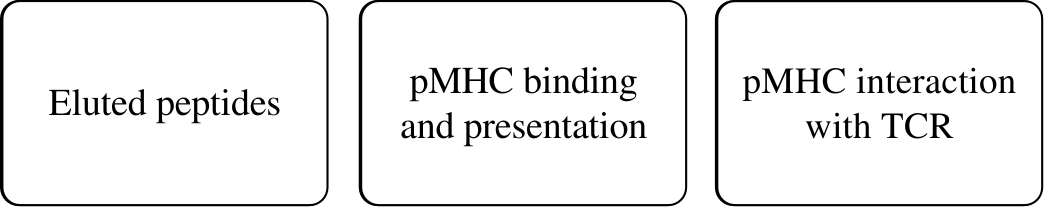
\includegraphics[width=8cm]{img/approaches} 
	\caption{The three phases and approaches that researches focus in the problem of neoantigen detection.}
	\label{fig:approaches}
\end{figure}


\subsection{Peptide-MHC (pMHC) binding and presentation}

Not all peptides eluted from tumor mutations are neoantigens; it depends on which peptides could bind to MHC. So, several works focus on peptide-MHC binding (pMHC). Moreover, there are three types of MHC: MHC class I, class II and class III. In human cells, they are named Human Leukocyte Antigen (HLA); for MHC class I, we have HLA-A, HLA-B, and HLA-C; and for MHC class II, HLA-DR, HLA-DQ, and HLA-DP \cite{neefjes2011towards}. \\

Most works focus in pMHC class I, because there is a lot of data, and the problem is not too complicated. The pMHC class I, represent a problem where a 9-mer peptide could bind to a MHC class I. In the other hand, the prediction of peptide MHC class II binding is challenging because the peptides are larger (normally 15-mer) and it binds to two amino acid chains in MHC class II.\\

The prediction of peptide-MHC binding usually refers to when a peptide bind to the MHC inside a nucleic cell. However, peptide-MHC presentation refers to the peptides that are presented by MHC in the membrane of cells. For instance, the process for peptide MHC binding and presentation is: first, antigens are degraded by the proteasome; then, the resulting peptides are translocated via a transporter associated with antigen presentation (TAP) into the endoplasmic reticulum (ER) and loaded onto MHC (peptide MHC binding); then, peptide–MHC class I complexes are released from the ER and transported via the Golgi to the plasma membrane (peptide MHC presentation); finally, the peptide-MHC is presented to TCR \cite{neefjes2011towards} (see Figure \ref{fig:mhc1_}). So, peptide-MHC binding (pMHC) and peptide-MHC presentation are two problems because not all pMHC are presented in the membrane \cite{mill2022neoms, de2020neoantigen, mill2022neoms, bulik2019deep, bassani2015mass, yadav2014predicting}. \\

\begin{figure}[H]
	\centering
	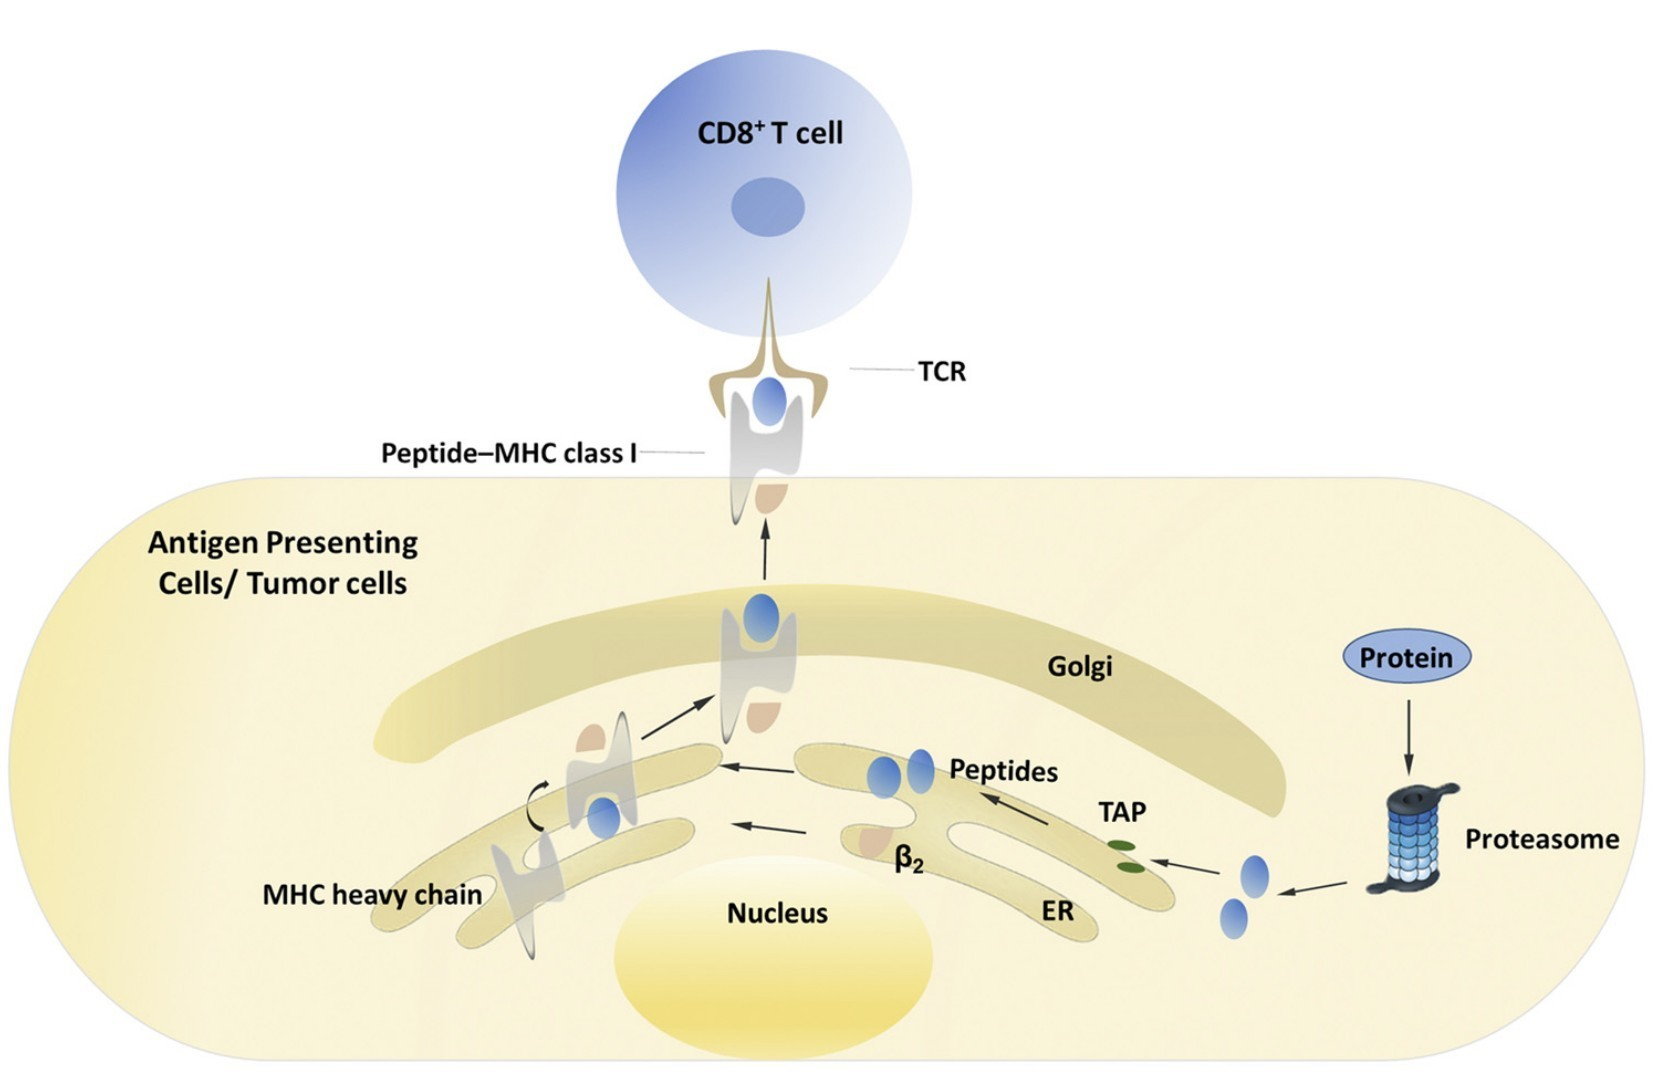
\includegraphics[width=0.4\textwidth]{img/neoantigen/mhc1.jpg}
	\caption{Peptide presentation by MHC class I. Source: \cite{zhang2019application}}
	\label{fig:mhc1_}
\end{figure}

In this section, we analyzed all research that used deep learning techniques for peptide-MHC binding and peptide-MHC presentation. Moreover, we divided the deep learning techniques in Convolutional Neural Networks (CNN), Recurrent Neural Networks (RNN), Transformers, and classic machine learning methods.\\

\subsubsection{CNN}

Convolutional Neural Networks (CNN) have been used in a range of different fields like computer vision, speech recognition, face recognition, object detection, etc. \cite{alzubaidi2021review}. Moreover, CNNs, are helpful because they notably reduce the number of parameters and enhance generalization. CNNs are regularly used in computer vision because they extract local spatial features and combine them with higher-order features \cite{marais2020leveraging}.\\

Several works apply CNNs for peptide-MHC binding and presentation. They differ in how they compute the inputs (amino acid sequences). Typically, they use one-hot encoding or BLOSUM to vectorize each amino acid, then join each vector and build a matrix that could be managed like an image. In Table \ref{tab:cnn1}, we present a list of the most recent works that use CNNs for neoantigen detection; we include the method used for encoding amino acids, what type of MHC class they focus and a link to the repository and database used for the experiments. Also, we distinguish if the research is used for pMHC binding or pMHC presentation. \\



\begin{table}[]
	\caption{List of research since 2018 that uses CNNs for peptide-MHC binding and presentation.}
	\label{tab:cnn1}
	\setlength{\tabcolsep}{0.5em} % for the horizontal padding
	{\renewcommand{\arraystretch}{1.2}% for the vertical padding
		
		\begin{tabular}{p{1.3cm}p{1.6cm}p{2cm}p{1.6cm}p{1.9cm}p{4cm}}
			\textbf{Ref.}                              & \textbf{Approach}        & \textbf{Name} & \textbf{MHC class} & \textbf{Encoding}                                   & \textbf{Description}                                                                                                                                                                                  \\ \hline
			
				\cite{you2022deepmhcii}	& peptide-MHC binding &	DeepMHCII &	MHC class-II &	Binding core and Peptides Flanking Regions (PFR), sequences and interactions between a peptide and an MHC-II molecule	& Uses a Binding Interaction Convolutional Layer (BICL) in order to get the representation of the interaction between peptides and MHC-II. \\
			
			 \cite{li2021deepimmuno}   & peptide-MHC binding      & DeepImmuno    & MHC class-I        & AAindex1 database                                   & The authors evaluated several machine learning methods, CNN got the best restults.            \\
			           \cite{lang2021neofox}     & peptide-MHC presentation & APPM          & MHC class-I        & One-hot encoding                                    & Three parallel CNN with MS data.                                       \\
			           \cite{lee2021connecting}  & peptide-MHC presentation & MHCfovea      & MHC class-I        & One-hot encoding                                    & Clusters N-terminal and C-terminal sub-motifs on observed and unobserved alleles, then MHCfovea calculated the hyper-motifs in order to disclose the relation between binding motifs and MHC-I                                                                        \\
			           \cite{junet2021cnn}       & peptide-MHC binding      & CNN-PepPred   & MHC class-II       & BLOSUM                                              & CNN is used to know motifs in peptide-MHC complexes.     \\
			           \cite{pei2020iconmhc}     & peptide-MHC binding      & IConMHC       & MHC class-I        & PCA of Aminoacid interaction from AAindex3 database & Learns from physical and chemical interaction properties between pairwise amino acids from the two molecules.                \\
			          \cite{saxena2020onionmhc} & peptide-MHC binding      & OnionMHC      & MHC class-I        & BLOSUM and structural features                      & Utilized complex structure and the peptide sequence features to predict the binding affinity of peptides to HLA-A*02:01                   -                                                                              \\
			           \cite{ng3704016minerva}   & peptide-MHC presentation & MINERVA       & MHC class-I        & physicochemical properties                          & The model learned the determinants of peptideMHC presentation, then they utilized these features to understand the impact of mutations on neoantigen presentation.                                                               \\
			           \cite{zhao2019peptide}    & peptide-MHC binding      & CNN-NF        & MHC class-I        & Sequence, Hydropathy index, Polarity, Length        & The authors used a novel set of features based on chemical properties. Moreover, they trained 193 models for each MHC.                                    \\
			           \cite{liu2019deepseqpan}  & peptide-MHC binding      & DeepSeqPan    & MHC class-I        & One-hot encoding                                    & The author comment that their model is universal and can be adapted to similar problems.                                  \\
			           \cite{han2018deep}        & peptide-MHC binding      & ConvMHC       & MHC class-I        & Contact side HLA.peptide                            & A novel image-like array (ILA) is presented to encode peptide sequences.                              
		\end{tabular}
	}
\end{table}



Furthermore, CNNs could be used with RNNs to improve generalization, or even we could include attention mechanisms. In this context, in Table \ref{tab:cnn1}, we present a list of works that used modified CNNs architectures. For instance, the first three rows detail the proposals with CNNs and attention mechanisms: DeepNetBim \cite{yang2021deepnetbim}, DeepAttentionPan \cite{jin2021deep} and ACME \cite{hu2019acme}. Then, in the last row, we describes MHCherryPan \cite{xie2020mhcherrypan}, which combines CNNs and RNNs.\\

\begin{table}[]
	\caption{List of research since 2018 that uses CNNs s with RNN or attention mechanisms for peptide-MHC binding and presentation.}
	\label{tab:cnn2}
	\setlength{\tabcolsep}{0.5em} % for the horizontal padding
	{\renewcommand{\arraystretch}{1.2}% for the vertical padding
		
		\begin{tabular}{p{1.3cm}p{1.6cm}p{2cm}p{1.6cm}p{1.9cm}p{4cm}}
			\textbf{Ref.}                              & \textbf{Approach}   & \textbf{Name}    & \textbf{MHC class} & \textbf{Encoding} & \textbf{Description}                                            \\ \hline
			         \cite{yang2021deepnetbim} & peptide-MHC binding & DeepNetBim       & MHC class-I        & BLOSUM            & Stands for binding and immunogenecity prediction with a CNN and an attention mechanism to make the final prediction. Encode data using BLOSUM50         \\
			
			           \cite{jin2021deep}        & peptide-MHC binding & Deep Attention Pan & MHC class-I        & BLOSUM            & Uses CNN with a attention mechanism and uses 20 trained netowrks to stabilize prediction performance. Morover, they used BLOSUM62 to encode input data.            \\
			
			           \cite{hu2019acme}         & peptide-MHC binding & ACME             & MHC class-I        & BLOSUM     & They used CNN with attention mechanism to extract interpretable binding patterns. For instance, this module assigned  weights to the feature vectors (residue positions) and then computed their weighted average to facilitate prediction Moreover, each amino acid is decoded using BLOSUM50.  \\
			
			           \cite{xie2020mhcherrypan} & peptide-MHC binding & MHCherryPan      & MHC class-I        & BLOSUM            & Combines CNN and RNN in order to deal with any length peptide sequences. it can be used in RNA-protein, DNA-protein, and RNA-DNA binding prediction.      
		\end{tabular}
	}
\end{table}


\subsubsection{RNN}

%%%%%%%%%%%%%%%%%%%%%%%%%%%%%%%%%%%%%%%%%%%%%%%%%%%%%%%%%%%%%%%%%%%
% Falta describir un pcoo de la historia de las RNN

In Table \ref{tab:rnn1}, we present a list of most recent works that uses RNNs for peptide-MHC binding and presentation prediction. For instance, in this case there works that used RNN with attentions mechanisms: MATHLA \cite{ye2021mathla}, DeepSeqPanII \cite{liu2021deepseqpanii} and DeepHLApan \cite{wu2019deephlapan}. There is also a works that uses standalone RNN, like a GRU model \cite{heng2021simple}, MHCnuggets which used a LSTM, and BVLSTM-MHC which used a  bilateral and variable long short-term memory (BVLSTM).  \\


\begin{table}[]
	\caption{List of research since 2018 that uses RNNs for peptide-MHC binding and presentation.}
	\label{tab:rnn1}
	\setlength{\tabcolsep}{0.5em} % for the horizontal padding
	{\renewcommand{\arraystretch}{1.2}% for the vertical padding
		
		\begin{tabular}{p{1.3cm}p{1.6cm}p{2cm}p{1.6cm}p{1.9cm}p{4cm}}
		\textbf{Ref.}                               & \textbf{Approach}   & \textbf{Name} & \textbf{MHC class} & \textbf{Encoding}           & \textbf{Description}                                                                                                                                                                                                                       \\
			          \cite{ye2021mathla}        & peptide-MHC binding & MATHLA        & MHC class-I        & BLOSUM                      & Integrates bi-directional long short-term memory network and multiple head attention mechanism. The model got good results for large ligand sequecences (11 to 15 amino acids)                    \\
			
			           \cite{liu2021deepseqpanii} & peptide-MHC binding                     & DeepSeqPanII                      & MHC class-II       & One-hot encoding and BLOSUM & It is a LSTM with attention mechanism, it have three parts:  sequence encoders, binding context extractor, and affinity predictor.                                                        \\
			
			           \cite{heng2021simple}      & peptide-MHC binding                     & GRU-based RNN                     & MHC class-II       & Embeding layer              & The autors uses a GRU model and present represent each sequence using an embeding layer which outputs 128 dim vectors.                                                                  \\
			
			           \cite{jiang2021predicting} & peptide-MHC binding                     & BVLSTM-MHC                        & MHC class-I        & One-hot encoding and BLOSUM & Review of current methods for predecting peptide-MHC-I binding problem. Moreover, the autors developed a bilateral and variable long short-term memory (BVLSTM).                                                                       \\
			
			           \cite{shao2020high}        & peptide-MHC binding                     & MHCnuggets                        & MHC class-I and II & Onehot encoding             & It uses a a long short-term memory (LSTM) model. Aditionally, the autors processed 26.3 million allele-peptide comparisons yielding 101,326 unique predicted immunogenic missense mutations (IMM)  \\
			
			           \cite{wu2019deephlapan}    & peptide-MHC binding                     & DeepHLApan                        & MHC class-I        & Onehot encoding             & Uses a Bidirectional Gated Recurrent Unit (BiGRO) with attention mechanism. The model got good results on unseen HLA alleles.                                       
		\end{tabular}
	}
\end{table}

\subsubsection{Transformers}

Tue attention mechanism was first proposed by Bahdanau in 2014 \cite{bahdanau2014neural}, in order to resolve the bottleneck problem using a fixed-length encoding vector. With this new approach, the authors got comparable state-of-art results for English to French translation. Then, this attention mechanism is used for natural language inference \cite{parikh2016decomposable}, and a structured attention networks is proposed \cite{kim2017structured}. Nevertheless, these attentions modules are commonly used in conjunction with a recurrent network. Then, in 2017, the paper: ``Attention Is Al You Need'' \cite{vaswani2017attention}, proposed a new network architecture (Transformer) base solely on attention mechanisms. \\

%%%%%%%%%%%%%%%%%%%%%%%%%%%%%%%%%%%%%%%%%%%%%%%%%%%%%%%%%%%%%%%%%%%
% aqui falta una descripcion de como trabaja las redes tranformer.


In Table \ref{tab:transformes}, we present a list of four works that recently used a transformer network in peptide-MHC binding and presentation. The majority of them uses a BERT architecture \cite{devlin2018bert}, which stands for a bidirectional transformer for language representation. For instance, we have 

\begin{table}[]
	\caption{List of research since 2018 that uses Transformers (self-attention) for peptide-MHC binding and presentation.}
	\label{tab:transformes}
	\setlength{\tabcolsep}{0.5em} % for the horizontal padding
	{\renewcommand{\arraystretch}{1.2}% for the vertical padding
		
		\begin{tabular}{p{1.3cm}p{1.6cm}p{2cm}p{1.6cm}p{1.9cm}p{4cm}}
			 \textbf{Ref.}                                  & \textbf{Approach}        & \textbf{Name} & \textbf{MHC class} & \textbf{Encoding}                  & \textbf{Description}                                                                                                                                                                                              \\
			           \cite{wang2022mhcroberta}     & peptide-MHC binding      & MHCRoBERTa    & MHC class-I        & Tokenized from a pre-trained model & The problem is resolve like a NLP approach. Moreover, they used transfer learning. This work outperformed NetMHCPan 3.0.                                                                                          \\
			           \cite{chu2022transformer}     & peptide-MHC binding      & TransPHLA     & MHC class-I        & Character embedding model          & The autors used a character embedding model to vectorize each amino acid. They used self-attention mechanism based in four blocks: the embedding block, encoder block, feature optimization block, encoder block. \\
			           \cite{cheng2021bertmhc}       & peptide-MHC binding      & BERTMHC       & MHC class-II       & Embeding layer                     & The autors used the pre-trained model TAPE to embed each aminoacid into a 768-dimensional vector. The self-attention mechanism learns the interaction of all possible amino acid pairs in the input sequence      \\
			           \cite{gasser2021interpreting} & peptide-MHC presentation & ImmunoBERT    & MHC class-I        & Embeding layer                     & They used TAPE as the embedding layer. Also, The autors used SHAP and LIME to analize the results and they concluded that N- and C-terminals are highly relevant.                                                
		\end{tabular}
	}
\end{table}


\subsection{\textit{Pipelines}}

Debido a la complejidad del proceso y la gran cantidad de métodos desarrollados, se ha desarrollado software y \textit{pipelines} que pretenden facilitar el uso de estas herramientas. Entre los \textit{pipelines} más conocidas antes del 2018 tenemos: Somaticseq \citep{fang2015ensemble}, CloudNeo \citep{bais2017cloudneo}, MuPeXI \citep{bjerregaard2017mupexi}, NeoepitopePred \citep{tran2015immunogenicity}, y NeoFuse \citep{gros2016prospective}. Estas herramientas en su mayoría toman como entrada archivos Variant Calling Files (VCF) y archivos de alineamiento BAM, para la detección de mutaciones (inserciones, eliminaciones y fusión de genes) y posibles neo antígenos. Luego, también hemos detallado, un conjunto de herramientas a partir del 2018, en la Tabla \ref{tab:review_pipelines}.




\begin{table}[H]
	\caption{Listado de \textit{pipelines} desde el 2018, para la detección de neo antígenos.}
	\label{tab:review_pipelines}
	\begin{tabular}{lp{2.5cm}p{4cm}p{4cm}}
		\textbf{Nombre} & \textbf{Autor-año}                                  & \textbf{Entrada}                                         & \textbf{Salida}                                     \\ \hline
		Neopepsee       & \cite{kim2018neopepsee}           & RNA-seq, somatic mutations (VCF), tipo de HLA (opcional) & Neo antígenos y niveles de expresión de los genes   \\
		PGV Pipeline    & \cite{rubinsteyn2018computational}& DNA-seq                                                  & Neo antígenos                                       \\
		ScanNeo         & \cite{wang2019scanneo}            & RNA-seq                                                  & Neo antígenos                                       \\
		NeoPredPipe     & \cite{schenck2019neopredpipe}     & Mutaciones (VCF) y tipo de HLA                           & Neo antígenos y anotación de variantes              \\
		pVACtools       & \cite{hundal2020pvactools}        & Mutaciones (VCF)                                         & Neo antígenos                                       \\
		ProGeo-neo      & \cite{li2020progeo}               & RNA-seq y somatic mutations (VCF)                        & Neo antígenos                                       \\
		neoepiscope     & \cite{wood2020neoepiscope}        & Somatic mutations (VCF) y archivos BAM                   & Neo antígenos y mutaciones                          \\
		neoANT-HILL     & \cite{coelho2020neoant}           & RNA-seq y somatic mutations (VCF)                        & Neo antígenos,  y niveles de expresión de los genes \\
		NAP-CNB         & \cite{wert2021predicting}         & RNA-seq                                                  & Neo antígenos                                       \\
		Valid-NEO       & \cite{terai2022valid}             & Somatic mutations (VCF), tipo de HLA (opcional)          & Neo antígenos                                      
	\end{tabular}
\end{table}


\subsection{\textit{Bases de datos}}

En la Tabla \ref{tab:bd}, presentamos una lista de bases de datos públicas. Estas bases de datos se centran en la interacción \textit{peptide-MHC} \citep{wu2018tsnadb, zhou2019neopeptide, tan2020dbpepneo, lu2022dbpepneo2} y pMHC con TCR \citep{shugay2018vdjdb, bagaev2020vdjdb}. También, hay un trabajo que presenta las estructuras 3D de las péptidos y HLA abriendo una nueva rama de investigación desde otro enfoque. Finalmente, la base de datos por excelencia IEDB \citep{vita2019immune}.



\begin{table}[H]
	\caption{Bases de datos públicas de \textit{pMHC binding}, \textit{pMHC presentation}, interacción pMHC-TCR y estructuras 3D de proteínas.}
	\label{tab:bd}
	\begin{tabular}{lp{3cm}p{8cm}}
		\textbf{Nombre} & \textbf{Autor-año}                                                                & \textbf{Descripción}                                                                                                                                                                                      \\ \hline
		VDJdb           & \cite{shugay2018vdjdb} y \cite{bagaev2020vdjdb}& Base de datos del enlace TCR con pMHC, cuenta con 5491 muestras                                                                                                                                           \\
		IEDB            & \cite{vita2019immune}                                           & La base de datos mas grande, contiene información \textit{T-cell epitopes} de humanos y otros organismos.                                                                                                          \\
		TSNAdb          & \cite{wu2018tsnadb}                                             & Contiene 7748 muestras de mutaciones y HLA de 16 tipos de Cáncer.                                                                                                                                         \\
		NeoPeptide      & \cite{zhou2019neopeptide}                                       & Contiene muestras de neo antígenos, resultado de mutaciones somáticas y artículos relacionados. Contiene 1818137 epitopes de ms de 36000 neo antígenos.                                                   \\
		pHLA3D          & \cite{e2019phla3d}                                              & Presenta 106 estructuras 3D de las cadenas alpha, $\beta_2M$ y peptidos de las moléculas HLA-I                                                                                                               \\
		dbPepNeo        & \cite{tan2020dbpepneo}                                          & Tiene muestras validadas del enlace \textit{peptide-MHC}, a partir de MS. Contiene 407794 muestras de baja calidad, 247 de mediana calidad y 295 muestras de alta calidad.                                         \\
		dbPepNeo2. 0    & \cite{lu2022dbpepneo2}                                          & Recolecta una lista de neo antígenos y moléculas HLA. Presenta 801 muestras de alta calidad y 842289  de mala calidad de HLAs. Tambien, 55 neo antígenos de clase II y 630 neo antígenos enlazados a TCR. \\
		
		IntroSpect      & \cite{zhang2022introspect}                                      & Herramienta para la construcción de bases de datos sobre \textit{peptide-MHC binding} . Utiliza datos de \textit{Mass Spectrometry}     \\
		
		IPD-IMGT/HLA & \cite{robinson2020ipd}    &             Tiene secuencias de moléculas MHC, 25000 alleles de 45 genes.                                                                                     
	\end{tabular}
\end{table}


%%%%%%%%%%%%%%%%%%%%%%%%%%%%%%%%%%%%%%%%%%%%%%%%%%%%%%%%%%%%%%%%%%%%%%%%%%%%%%%%%%%
%%%%%%%%%%%%%%%%%%%%%%%%%%%%%%%%%%%%%%%%%%%%%%%%%%%%%%%%%%%%%%%%%%%%%%%%%%%%%%%%%%%
%%%%%%%%%%%%%%%%%%%%%%%%%%%%%%%%%%%%%%%%%%%%%%%%%%%%%%%%%%%%%%%%%%%%%%%%%%%%%%%%%%%
%%%%%%%%%%%%%%%%%%%%%%%%%%%%%%%%%%%%%%%%%%%%%%%%%%%%%%%%%%%%%%%%%%%%%%%%%%%%%%%%%%%

\subsection{\textit{Reviews}}

%%%%%%%%%%%%%%%%%%%%%%%%%%%%%%%%%%%%%%%%%%%%%%%%%%%%%%%%%%%%%%%%%%%%%%%%%%%%%%%%%%%
%%%%%%%%%%%%%%%%%%%%%%%%%%%%%%%%%%%%%%%%%%%%%%%%%%%%%%%%%%%%%%%%%%%%%%%%%%%%%%%%%%%
%%%%%%%%%%%%%%%%%%%%%%%%%%%%%%%%%%%%%%%%%%%%%%%%%%%%%%%%%%%%%%%%%%%%%%%%%%%%%%%%%%%
%%%%%%%%%%%%%%%%%%%%%%%%%%%%%%%%%%%%%%%%%%%%%%%%%%%%%%%%%%%%%%%%%%%%%%%%%%%%%%%%%%%

La detección de neo antígenos es un problema interdisciplinar y esto ha originado  varios \textit{reviews} desde diferentes perspectivas. Entonces se ha planteado la siguiente clasificación: basados en \textit{Next-Generation Sequencing}, \textit{Mass Spectrometry}, interacción \textit{peptide-MHC}, basados en información estructural, enfocados en TCR, buenas prácticas y los enfocados en el proceso completo de generación de vacunas personalizadas.

Primero, presentamos los trabajos que se enfocan en estudios de \textit{Next-Generation Sequencing} (Tabla \ref{tab:review_seq}), para la detección de neo antígenos e inmunoterapia del Cáncer. Estos trabajos principalmente utilizan información secuencial de \textit{DNA} y gracias a las tecnologías modernas ahora se pueden considerar las secuencias de \textit{RNASeq}. Las tecnologías de RNASeq, proveen información mas precisa de la transcripción e identificación de isoformos que otros métodos \citep{wang2009rna}. Mayormente, estas tecnologías se limitan a algoritmos alineamiento con genomas de referencia \citep{groisberg2018immunotherapy}. 




%%%%%%%%%%%%%%%%%%%%%%%%%%%%%%%%%%%%%%%%%%%%%%%%%%%%%%%%%%%%%%%%%%%%%%%%%
%PENDIENTE queda pendinete agregar ms información
%%%%%%%%%%%%%%%%%%%%%%%%%%%%%%%%%%%%%%%%%%%%%%%%%%%%%%%%%%%%%%%%%%%%%%%%%

\begin{table}[H]
		\caption{Listado de los \textit{reviews}, que se enfocan en estudios de \textit{Next-Generation Sequencing} para la detección de neo antígenoes e inmunoterapia del Cáncer.}
	\label{tab:review_seq}
	\begin{tabular}{p{3cm}p{10cm}}
	\textbf{Autor-año }                            & \textbf{Título}                                                                                                                                \\ \hline
		\cite{zhou2022comprehensive}     & A Comprehensive Survey of Genomic Mutations in Breast Cancer Reveals Recurrent Neoantigens as Potential Therapeutic Targets            \\
		\cite{battaglia2020neoantigen}   & Neoantigen prediction from genomic and transcriptomic data                                                                             \\
		\cite{mirandola2020quest}        & The Quest for the Next-Generation of Tumor Targets: Discovery and Prioritization in the Genomics Era                                   \\		
		\cite{groisberg2018immunotherapy}& Immunotherapy and next-generation sequencing guided therapy for precision oncology: what have we learnt and what does the future hold?
	\end{tabular}
\end{table}

Algunos trabajos son más específicos, y se enfocan en la interacción de un péptido y la molécula MHC. Esta interacción es un factor clave, porque si se forma el enlace pMHC y luego este compuesto es presentado a las células T, es posible activar el sistema inmune. En la Tabla \ref{tab:review_mhc}, se presenta estos \textit{reviews}. La mayoría de estos trabajos, se centran en la molécula MHC-I \citep{mateo2020comparison, mei2020comprehensive, schmidt2019mhc, mei2020comprehensive} , molécula MHC-II \citep{jensen2018improved} y todos los tipos de MHC en general \citep{nielsen2020immunoinformatics, liu2020review, liu2020review}. También, hay trabajos que estudian la complejidad de esta molécula y todos sus \textit{alleles} \citep{radwan2020advances}.



\begin{table}[H]
	\caption{Listado de los \textit{reviews}, que se enfocan en estudios de la interacción de péptidos y la molécula MHC, para la detección de neo antígenoes.}
	\label{tab:review_mhc}
	\begin{tabular}{p{3cm}p{10cm}}
		\textbf{Autor-año }                            & \textbf{Título}                                                                                                                                \\ \hline
		\cite{mateo2020comparison}          & Comparison of machine learning models for the prediction of cancer cells using MHC class I complexes                 \\
		\cite{mei2020comprehensive}         & A comprehensive review and performance evaluation of bioinformatics tools for HLA class I peptide-binding prediction \\
		
		\cite{nielsen2020immunoinformatics} & Immunoinformatics: predicting peptide–MHC binding                                                                    \\
		\cite{liu2020review}                & A review on the methods of peptide-MHC binding prediction                                                            \\
		\cite{paul2020major}                & Major histocompatibility complex binding, eluted ligands, and immunogenicity: benchmark testing and predictions      \\
	
		\cite{radwan2020advances}           & Advances in the Evolutionary Understanding of MHC Polymorphism 
		
		                                                      \\
		
		\cite{schmidt2019mhc}               & MHC class I presented antigens from malignancies: A perspective on analytical characterization \& immunogenicity     \\
	
		\cite{jensen2018improved}           & Improved methods for predicting peptide binding affinity to MHC class II molecules                                   \\
		
		\cite{mei2020comprehensive}         & A comprehensive review and performance evaluation of bioinformatics tools for HLA class I peptide-binding prediction \\
		\cite{liu2020review}                & A review on the methods of peptide-MHC binding prediction                                                            \\
		\cite{paul2020major}                & Major histocompatibility complex binding, eluted ligands, and immunogenicity: benchmark testing and predictions      \\
		\cite{radwan2020advances}           & Advances in the Evolutionary Understanding of MHC Polymorphism                                                       \\
		\cite{schmidt2019mhc}               & MHC class I presented antigens from malignancies: A perspective on analytical characterization \& immunogenicity     \\
		\cite{jensen2018improved}           & Improved methods for predicting peptide binding affinity to MHC class II molecules                                  
	\end{tabular}
\end{table}

La mayoría de \textit{reviews} estudian las técnicas basadas en secuencias de DNA y RNA, pero recientemente se está utilizando \textit{Mass spectrometry}, para secuenciar los péptidos y moléculas MHC ya enlazados y presentes en las membranas de las células. Este avance ha impulsado la creación de nuevas bases de datos y métodos para el problema de \textit{peptide-MHC presentation}. En este contexto, en la Tabla \ref{tab:review_ms}, se presentan todos los \textit{reviews}, enfocados en estudiar \textit{Mass spectrometry} para la detección de neo antígenos.



\begin{table}[H]
	\caption{Listado de los \textit{reviews}, que se enfocan en estudios de \textit{Mass spectrometry} para la detección de neo antígenoes.}
	\label{tab:review_ms}
	\begin{tabular}{p{3cm}p{10cm}}
	\textbf{Autor-año }                            & \textbf{Título}                                                                                                                                 \\ \hline
		\cite{kote2020mass}           & Mass spectrometry-based identification of MHC-associated peptides                                                          \\
		\cite{kote2020mass}           & Mass spectrometry-based identification of MHC-associated peptides                                                          \\
		\cite{zhang2019application}   & Application of mass spectrometry-based MHC immunopeptidome profiling in neoantigen identification for tumor immunotherapyA \\
		\cite{chen2021identification} & Identification of MHC peptides using mass spectrometry for neoantigen discovery and cancer vaccine development             \\
		\cite{creech2018role}         & The role of mass spectrometry and proteogenomics in the advancement of HLA epitope prediction                              \\
		\cite{zhang2019application}   & Application of mass spectrometry-based MHC immunopeptidome profiling in neoantigen identification for tumor immunotherapyA \\
		\cite{creech2018role}         & The role of mass spectrometry and proteogenomics in the advancement of HLA epitope prediction                             
	\end{tabular}
\end{table}


En si la detección de neo antígenos, es un proceso muy largo e integra métodos de secuenciamiento, alineamiento, detección de mutaciones, identificación de péptidos, predicción de la interacción \textit{peptide-MHC}, y finalmente el trabajo biotecnológico para la generación de vacunas. Entonces, en la Tabla \ref{tab:review_2022_2021} y \ref{tab:review_2020_2019}, se presenta el lista de \textit{reviews}, que explican el problema de generación de vacunas pero desde una vista panoramica incluyendo todo el proceso completo. Algunos trabajos se enfocan en demostrar la posibilidad de crear vacunas personalizadas contra en Cáncer \citep{lang2022identification, richard2022neoantigen, pao2022therapeutic, reynolds2022neoantigen, mccaffrey2022bioinformatic, fritsch2020personal} y otros trabajos, priorizan la importancia de los neo antígenos \citep{okada2022identification, zheng2022neoantigen, wang2021gene, pearlman2021targeting, arnaud2020biotechnologies, han2020progress}.


\begin{table}[H]
	\caption{Listado de los \textit{reviews}, que se enfocan en presentar en proceso general de detección de neo antígenoes y vacunas personalizadas del año 2022 y 2021.}
	\label{tab:review_2022_2021}
	\begin{tabular}{p{3cm}p{10cm}}
		\textbf{Autor-año }                            & \textbf{Título}                                                                                                                             \\ \hline
		\cite{tran2022tale}                   & A tale of solving two computational challenges in protein science: neoantigen prediction and protein structure prediction                 \\
		\cite{lang2022identification}         & Identification of neoantigens for individualized therapeutic cancer vaccines                                                              \\
		\cite{okada2022identification}        & Identification of Neoantigens in Cancer Cells as Targets for Immunotherapy                                                                \\
		\cite{bollineni2022chasing}           & Chasing neoantigens; invite naïve T cells to the party                                                                                    \\
		\cite{richard2022neoantigen}          & Neoantigen-based personalized cancer vaccines: the emergence of precision cancer immunotherapy                                            \\
		\cite{pao2022therapeutic}             & Therapeutic Vaccines Targeting Neoantigens to Induce T-Cell Immunity against Cancers                                                      \\
		\cite{fang2022neoantigens}            & Neoantigens and their potential applications in tumor immunotherapy                                                                       \\
		\cite{zheng2022neoantigen}            & Neoantigen: A Promising Target for the Immunotherapy of Colorectal Cancer                                                                 \\
		\cite{redwood2022s}                   & What's next in cancer immunotherapy?-The promise and challenges of neoantigen vaccination                                                 \\
		\cite{reynolds2022neoantigen}         & Neoantigen Cancer Vaccines: Generation, Optimization, and Therapeutic Targeting Strategies                                                \\
		\cite{roesler2022beyond}              & Beyond Sequencing: Prioritizing and Delivering Neoantigens for Cancer Vaccines                                                            \\
		\cite{mccaffrey2022bioinformatic}     & Bioinformatic Techniques for Vaccine Development: Epitope Prediction and Structural Vaccinology                                           \\
		\cite{fotakis2021computational}       & Computational cancer neoantigen prediction: current status and recent advances                                                            \\
		\cite{wang2021beyond}                 & Beyond tumor mutation burden: tumor neoantigen burden as a biomarker for immunotherapy and other types of therapy                         \\
		\cite{ferreira2021glycoproteogenomics}& Glycoproteogenomics: Setting the Course for Next-generation Cancer Neoantigen Discovery for Cancer Vaccines                               \\
		\cite{blass2021advances}              & Advances in the development of personalized neoantigen-based therapeutic cancer vaccines                                                  \\
		\cite{wang2021gene}                   & Gene fusion neoantigens: Emerging targets for cancer immunotherapy                                                                        \\
		\cite{pearlman2021targeting}          & Targeting public neoantigens for cancer immunotherapy                                                                                     \\	                                                                    
	\end{tabular}
\end{table}

\begin{table}[H]
	\caption{Listado de los \textit{reviews}, que se enfocan en presentar en proceso general de detección de neo antígenoes y vacunas personalizadas del año 2020 y 2019.}
	\label{tab:review_2020_2019}
	\begin{tabular}{p{3cm}p{10cm}}
		\textbf{Autor-año }                            & \textbf{Título}                                                                                                                             \\ \hline	
		\cite{arnaud2020biotechnologies}      & Biotechnologies to tackle the challenge of neoantigen identification                                                                      \\
		\cite{fritsch2020personal}            & Personal neoantigen cancer vaccines: a road not fully paved                                                                               \\
		\cite{holtstrater2020bioinformatics}  & Bioinformatics for cancer immunotherapy                                                                                                   \\
		\cite{roudko2020computational}        & Computational prediction and validation of tumor-associated neoantigens                                                                   \\
		\cite{esprit2020neo}                  & Neo-antigen mRNA vaccines                                                                                                                 \\
		\cite{chen2020personalized}           & Personalized neoantigen vaccination with synthetic long peptides: recent advances and future perspectives                                 \\
		\cite{londhe2020personalized}         & Personalized neoantigen vaccines: A glimmer of hope for glioblastoma                                                                      \\
		\cite{han2020progress}                & Progress in neoantigen targeted cancer immunotherapies                                                                                    \\
		\cite{keshavarzi2020ai}               & AI and Immunoinformatics                                                                                                                  \\
		\cite{jiang2019tumor}                 & Tumor neoantigens: from basic research to clinical applications                                                                           \\
		\cite{mardis2019neoantigens}          & Neoantigens and genome instability: impact on immunogenomic phenotypes and immunotherapy response                                         \\
		\cite{de2019advancing}                & Advancing cancer immunotherapy: a vision for the field                                                                                    \\
		\cite{li2018recent}                   & Recent updates in cancer immunotherapy: a comprehensive review and perspective of the 2018 China Cancer Immunotherapy Workshop in Beijing \\
		\cite{sidhom2018applications}         & Applications of Artificial Intelligence \& Machine Learning in Cancer Immunology                                                          \\
		\cite{doytchinova2018silico}          & In silico prediction of cancer immunogens: current state of the art                                                                      
	\end{tabular}
\end{table}


Gracias a \textit{Next-generation Secuencing} y \textit{Mass spectrometry}, se ha logrado muchon avances en la Bioinformática, pero a veces es necesario tener información adicional como las propiedades estructurales de los aminoacidos. Debido a esto, han surgido varias investigaciones y los \textit{reviews} de la Tabla \ref{tab:review_structure}, que explican como se pueden utilizar este tipo de propiedades para predecir la interacción pMHC. Lamentablemente, solo se ha identificado dos trabajos \citep{perez2022structural,antunes2018structure}, porque no se cuenta con muchas muestras de este problema.



\begin{table}[H]
	\caption{Listado de los \textit{reviews}, que se enfocan en estudios que utilizan propiedades estructurales de los aminoacidos para la de detección de neo antígenoes.}
	\label{tab:review_structure}
	\begin{tabular}{p{3cm}p{10cm}}
		\textbf{Autor-año }                            & \textbf{Título}                                                                                                                             \\ \hline	
		\cite{perez2022structural}  & Structural Prediction of Peptide–MHC Binding Modes                                                 \\
		\cite{antunes2018structure} & Structure-based methods for binding mode and binding affinity prediction for peptide-MHC complexes \\		
	\end{tabular}
\end{table}


Generalmente, con la predicción del enlace pMHC, podría terminar el trabajo Bioinformático, para luego proceder a los trabajos \textit{in vitro} e \textit{in vivo}. Pero, algunos trabajos, tambien buscan entender que hace que un cmpuesto pMHC se enlace al TCR y así se genere una respuesta inmune. Esto tambien ha generado bastantes \textit{reviews} presentados en la Tabla \ref{tab:review_tcr}.

\begin{table}[H]
	\caption{Listado de los \textit{reviews}, que se enfocan en estudios de la interacción de compuestos pMHC con TCR.}
	\label{tab:review_tcr}
	\begin{tabular}{p{3cm}p{10cm}}
		\textbf{Autor-año }                            & \textbf{Título}                                                                                                                             \\ \hline
		\cite{kast2021advances}     & Advances in identification and selection of personalized neoantigen/T-cell pairs for autologous adoptive T cell therapies           \\
		\cite{schaap2021t}          & T Cell Epitope Prediction and Its Application to Immunotherapy                                                                      \\                                    
		\cite{zvyagin2020overview}  & An overview of immunoinformatics approaches and databases linking T cell receptor repertoires to their antigen specificity          \\
		\cite{sidney2020epitope}    & Epitope prediction and identification- adaptive T cell responses in humans                                                          \\
		
		\cite{zvyagin2020overview}  & An overview of immunoinformatics approaches and databases linking T cell receptor repertoires to their antigen specificity          \\
		\cite{spear2019understanding} & Understanding TCR affinity, antigen specificity, and cross-reactivity to improve TCR gene-modified T cells for cancer immunotherapy \\		                                               
		\end{tabular}
	\end{table}


Finalmente, se han desarrollado \textit{reviews} que detallan los principales desafíos, buenas prácticas y perspectivas futuras en la detección de neo antígenos (Tabla \ref{tab:review_buen}). De estos trabajos, el \textit{review} de \cite{gopanenko2020main} y \cite{borden2022cancer}, explican detalladamente, todos los métodos de cada fase para la detección de neo antígenos; adicionalmente, explican las ventajas de cada método y los problemas actuales. También, resaltamos el trabajo de \cite{richters2019best}, que resalta las buenas prácticas de este campo de estudio.




\begin{table}[H]
	\caption{Listado de los \textit{reviews}, que se enfocan en presentar buenas prácticas en el proceso de detección de neo antígenoes y generación de vacunas personalizadas,}
	\label{tab:review_buen}
	\begin{tabular}{p{3cm}p{10cm}}
		\textbf{Autor-año }                            & \textbf{Título}                                                                                                                                \\ \hline
		\cite{borden2022cancer}       & Cancer Neoantigens: Challenges and Future Directions for Prediction, Prioritization, and Validation                                           \\
		\cite{chen2021challenges}     & Challenges targeting cancer neoantigens in 2021: a systematic literature review                                                             \\	
		\cite{gopanenko2020main}      & Main strategies for the identification of neoantigens                                                                                         \\
		\cite{de2020neoantigen}       & Neoantigen prediction and computational perspectives towards clinical benefit: recommendations from the ESMO Precision Medicine Working Group \\	
		
		\cite{richters2019best}       & Best practices for bioinformatic characterization of neoantigens for clinical utility                                                         \\
		\cite{garcia2019determinants} & Determinants for Neoantigen Identification                                                                                                    \\
		\cite{aurisicchio2018perfect} & The perfect personalized cancer therapy: cancer vaccines against neoantigens                                                                  \\
		\cite{barros2018immunological}& Immunological-based approaches for cancer therapy                                                                                             \\
		\cite{tureci2018challenges}   & Challenges towards the realization of individualized cancer vaccines                                                                          \\
		\cite{villani2018systems}     & Systems immunology: Learning the rules of the immune system                                                                                   \\
		\cite{richters2019best}       & Best practices for bioinformatic characterization of neoantigens for clinical utility                                                         \\
		\cite{garcia2019determinants} & Determinants for Neoantigen Identification                                                                                                    	                                                               \\
		\cite{barros2018immunological}& Immunological-based approaches for cancer therapy                                                                                            \\	
	                                                                                
	\end{tabular}
\end{table}






